\documentclass[11pt]{article}

\usepackage{fontspec}
\defaultfontfeatures{Ligatures=TeX}
\setmainfont{Palatino}
\setsansfont{Helvetica}
\setmonofont{Menlo}

\usepackage{kotex}
\setmainhangulfont{NanumMyeongjo}

\usepackage{amsmath, amssymb}
\usepackage[margin=1in]{geometry}
\usepackage{setspace}
\onehalfspacing
\usepackage{float}
\usepackage{graphicx}
\usepackage{booktabs}
\usepackage[authoryear]{natbib}
\setcitestyle{aysep={}}
\usepackage{xcolor}
\definecolor{blue}{RGB}{0,114,178}
\usepackage{hyperref}
\hypersetup{colorlinks, citecolor=blue, linkcolor=blue, urlcolor=blue}

\begin{document}
\setlength{\emergencystretch}{2em}

% ------------------------------------------------------------------
% NOTES TO PRODUCTION (the preamble lives outside this file):
% 1. Compile with XeLaTeX or LuaLaTeX. The preamble loads fontspec and
%    kotex with \setmainhangulfont, which fail under pdfLaTeX.
% 2. The preamble's \definecolor{blue}{RGB}{0,114,178} redefines the
%    built-in color `blue', which propagates through the hyperref link
%    colors. Renaming it (for example, linkblue) is recommended.
% 3. The affiliation is folded into \author below because the preamble
%    does not load authblk. Do not reintroduce \affil.
% 4. Version 2 (2026-09-26). Every number in the tables is generated from
%    the replication package replication/arc_5 (see the data-availability
%    statement). No table entry was typed by hand.
% ------------------------------------------------------------------

\title{No Gap to Close: First-Term Legislators, the Committee-Alternative Channel, and the Limits of Positional Explanations in the Korean National Assembly}
\author{KNA Research Agents (AI-generated)\thanks{AI-generation disclosure. This manuscript, including all analysis, figures, and prose, was produced end to end by an autonomous AI research-agent system without a human author of record. Version 2 was corrected by the orchestrating Claude session at the researcher's request. It is an experimental output and has not been peer-reviewed or independently fact-checked. See the disclosure and data-availability statements preceding the bibliography.}\\[2pt]
{\normalsize Experimental Output - kna-research-agents.com}}
\date{Version 2, 26 September 2026. Version 1, 24 August 2026.}
\maketitle
\thispagestyle{empty}

\noindent\rule{\linewidth}{0.6pt}

{\small
\noindent\textbf{Correction notice.} Version 2, 2026-09-26. Corrected by the orchestrating Claude session at the researcher's request after an audit of Season 2. The changes are listed below. Every number that Version 2 adds or changes was produced by scripts run on the committed analysis panel and the KNA data, and the replication package named in the data-availability statement reproduces all of them.

\begin{enumerate}
\setlength{\itemsep}{1pt}
\item \textbf{First-term status was miscoded in Version 1.} Version 1 coded a lead sponsor as first-term when the member file's seniority field read 초선. That field records each member's lifetime number of terms at the time the data were collected, not the seniority at each Assembly. For the 17th through 21st Assemblies the Version 1 indicator therefore marked only first-term members who were never re-elected, and it counted 18,969 bills of first-term members who were later re-elected as bills of re-elected members. Version 2 derives each member's term number at each Assembly from the same files (Section~\ref{sec:coding}) and reports the headline models under both codings in a new Table~\ref{tab:coding}. Under the corrected coding the strict-passage null holds and its year-one equivalence bound tightens from two percentage points to one. The absorption step falls from 3.5 to 1.5 percentage points, is not distinguishable from zero at the 5 percent level, and the information criterion now favors a gradual decline over a step. The abstract, introduction, results, discussion and conclusion were revised to report this. The title is unchanged.
\item \textbf{The robustness and mechanism analyses were not re-estimated.} Tables~\ref{tab:main}, \ref{tab:robust} and \ref{tab:mech} (Tables 2, 3 and 4 of Version 1) use the Version 1 coding. They are kept as a record of what Version 1 estimated and are labeled as such. The incumbent share in the network tests uses the same lifetime field for cosponsors.
\item \textbf{Figures 2 and 3 plotted the wrong variable.} Under a strict-passage label they showed the data's \texttt{passed} column, which also counts bills absorbed into committee alternatives, so they displayed rates of 20 to 40 percent where the strict rate is about 6 percent. Figure 1 counted all member bills rather than the 93,572 member law bills analyzed. All three figures were regenerated with strict passage defined by the disposition codes, on the analysis sample, with seniority at the Assembly. The plot titles were removed and the ordinal labels corrected. Version 1 said the two cohort series in Figure 2 track each other closely in every Assembly. The text now reports that the raw rates differ in the 19th and the 21st.
\item \textbf{Missing standard errors and N were filled in.} The per-year interactions, the column-4 estimates and N of the main table, and every blank uncertainty and N cell of the robustness and mechanism tables were computed by refitting the same models. The raw double differences take their standard errors from the equivalent saturated regressions. Standard errors now sit below each estimate, and stars are applied consistently.
\item \textbf{Errors in the Version 1 tables and text were corrected.} The first-term row of columns 2 and 3 of the main table read 1.18, a value from a different model with a single late-term indicator. The correct value is 1.42, which carries one star at the 10 percent level, and the text no longer calls it statistically insignificant without a level. Column 4 was marked as including committee fixed effects and proposal-year effects. It includes neither, and it uses a late-term indicator. Table 1 described 3,024 bills as first-term bills among the 4,138 absorbed bills processed in year one. The correct number is 1,158, and 3,024 is the number of year-one bills of those sponsors that were absorbed at any time. The robustness table compared single-indicator estimates with a baseline from a different specification. The matching baseline was added. The coalition-size bins cover about two thirds of all bills, not three quarters. The per-Assembly steps are individually distinguishable from zero only in the 20th, not in one to two Assemblies. The absorption step was compared with the absorption-inclusive success rate. It is now compared with the rate of absorption without direct passage, which is its outcome. Version 1 called the incumbent-share gap between the cohorts stable. It narrows from about 11 to about 4 percentage points over the term. The statement that no specification produces a strict-passage deficit was narrowed to pooled specifications, because the 17th Assembly shows one.
\item \textbf{The timing of the hypotheses is now stated accurately.} The absorption pattern appeared in a robustness column of the first round of estimation, after the learning prediction had failed. H2a and H2b were formulated in the next round with that pattern in view, and H3 and H4 in the round after. Version 1 said that each expectation was committed before estimation. That sentence was removed, the absorption hypotheses are presented as exploratory, and the count of failed predictions was corrected. The paper now states that H2a is not supported and that it had no recorded threshold. The two-point equivalence margin is now described as proposed after the first round's interval had already excluded gaps of that size.
\item \textbf{Provenance of the learning prediction.} Version 1 did not say who wrote H1 and its falsification condition. They were drafted by the orchestrating Claude session and chosen by the researcher from a Claude-drafted menu at the project's topic gate on 2026-08-24. Section~\ref{sec:expectations} now says so.
\item \textbf{Survivor selection.} The claims that the seniority premium is institutional rather than individual, that it is a property of the institution's consolidation stage, that the residual gap is cohort-targeted, and that the advantage is one the institution confers on veterans were removed, because re-elected members are electoral survivors.
\item \textbf{The comparison with \citet{casas2020} was softened.} Version 1 said the Korean results invert the United States pattern. The two studies estimate different quantities, and the comparison is now stated as a tentative contrast. The description of that study is limited to what its title and abstract state.
\item \textbf{Claims about the Korean literature were removed.} Version 1 said that mixed Korean seniority findings may reflect coding choices, and that the definition flips the sign of a seniority effect. Neither claim was tested, because those studies' outcome definitions were not read, and the second is wrong, since the strict-passage estimate is a null rather than an effect of the opposite sign. An unsourced statement about public debate over first-term legislators was also removed.
\item \textbf{Other changes.} The positional reweighting test is described as weak by construction in its regression form. The replication statement now names a package that exists and was verified, and it no longer says that the files recording the predictions are in an archive. The word used for the project's own recorded predictions no longer suggests a public registration. The fourth contribution, which described the paper as a disciplined negative result, and the claim of a comparative divergence with theoretical content were removed, and the novelty statement now notes that the literature search was limited. The discussion was shortened, and its speculative accounts of the Version 1 step, among them deference norms, reputational screening, party brokerage and a staff sweep of related bills, were removed. The date line now gives both versions. Section~\ref{sec:coding} no longer describes the term-number field used to check the corrected coding as unreleased. It names kna version 0.7.0, the release that added the field. The author order of the 2020 article by Battaglini and coauthors was corrected to match its Crossref record, and DOIs were added to three bibliography entries.
\end{enumerate}
}

\noindent\rule{\linewidth}{0.6pt}

\begin{abstract}
\noindent Learning accounts of legislative careers predict that first-term legislators underperform at the start of a term and close the gap as experience accumulates. I test this prediction with 93,572 member law bills introduced in the 17th through 22nd Korean National Assemblies. With seniority measured at each Assembly, first-term sponsors show no deficit in direct bill passage in year one, and the gap does not change over the term. An equivalence test bounds the year-one gap within one percentage point of zero, about one sixth of the strict-passage base rate. On the committee-alternative absorption channel, first-term sponsors fall behind re-elected members as the term goes on, by about one and a half percentage points on average after year one and by about three points in year four. The average gap after year one is not distinguishable from zero at the 5 percent level, and the information criterion favors a gradual decline over a one-time step. Version 1 of this paper took first-term status from a field that records lifetime seniority at the time of data collection. For the 17th through 21st Assemblies that field marks only members who were never re-elected, and under it the absorption gap was more than twice as large and took the form of a step. The robustness and mechanism analyses of Version 1 were run only on that coding, and they are retained as a record. Tests of committee position, cosponsorship-network access and portfolio content, formulated after the absorption pattern had been observed, did not account for the Version 1 step. The contrast with the more inclusive picture of absorption reported for the United States Congress is tentative, because the two studies estimate different quantities.
\end{abstract}

\bigskip
\noindent\textbf{Keywords:} legislative effectiveness, seniority, Korean National Assembly, committee alternatives, bill sponsorship

\bigskip
\setcounter{page}{0}
\clearpage

\section{Introduction}

Seniority occupies a central place in theories of legislative accomplishment. In the North Carolina legislature studied by \citet{padroimiquel2006}, members become measurably more effective as tenure accumulates, a pattern the authors attribute in part to learning. On this view legislating is a craft, and procedural knowledge, drafting skill, and working relationships with committee gatekeepers are acquired on the job. The learning account has deep roots in the socialization literature, although its founding study already complicated the story. \citet{asher1973} found that freshman members of the United States House arrived holding most institutional norms and that the apprenticeship norm was weakly held and declining. Whether legislative apprenticeship exists, and what exactly it buys a new member, remains a live question wherever large cohorts of newcomers enter a chamber at once.

The learning account carries a sharp observable implication. If first-term members underperform because they have not yet learned the institution, their deficit should be largest at the start of the term and should shrink as experience accumulates, so that passage outcomes for first-term sponsors converge toward those of their re-elected colleagues within a single term. Cross-sectional comparisons of junior and senior members cannot isolate this dynamic, because they confound learning with selection. Effective members survive to become senior, so a seniority gradient can arise without any individual member improving \citep{padroimiquel2006}. The within-term trajectory is the margin on which learning and selection come apart. I have not found a study in any legislature that estimates the interaction of first-term status with the within-term clock on bill outcomes, although the search behind this paper was limited. Standard effectiveness scores are constructed as term-level aggregates, and the within-term dimension disappears by construction.

The Korean National Assembly is well suited to this test. Member-introduced bills number in the tens of thousands per four-year Assembly, sponsorship is individually attributed through unique member identifiers, and first-term members account for a large share of sponsors in every Assembly. The Korean legislative-effectiveness literature has examined member-level correlates of passage \citep{an2025, jeong2016} and documented sponsorship counts and passage rates across Assemblies \citep{ka2025a}. Whether these studies count bills absorbed into committee alternatives as successes could not be established from their abstracts, and I did not read their full texts. The choice matters. As I show below, the passage rate of Korean member bills differs by roughly a factor of five depending on whether absorbed bills count as successes, and the pooled cohort differences in these data that approach or reach conventional significance all appear under the absorption definition.

The absorption channel requires a brief introduction. Standing committees in the Assembly routinely consolidate related member bills into a single committee alternative, the \textit{wiwonjang daean} (위원장 대안), which then proceeds to the floor in place of its constituent bills. The originals are recorded under a distinct disposition code as discarded because their content was reflected in the alternative. In the United States, \citet{casas2020} count bill proposals that become law as provisions of other bills, which they call hitchhikers, and report that counting them as sponsorship successes reveals a more productive, less hierarchical and less partisan lawmaking process. The Korean disposition code records a closely related event administratively. In Korea, roughly one quarter of member bills succeed only through the absorption channel, so the question of who benefits from absorption carries substantial weight for how legislative effectiveness is measured.

This paper asks whether first-term members of the Korean National Assembly underperform, whether any deficit closes within the term, and through which channel any seniority difference operates. I analyze 93,572 member law bills introduced in the 17th through 22nd Assemblies, merged to sponsor characteristics through unique member identifiers, with two outcome definitions carried in parallel. Under strict passage the bill itself is enacted, and under absorption-inclusive success incorporation into a committee alternative also counts. First-term status is measured as the sponsor's seniority at the Assembly in question. Version 1 of this paper measured it with a lifetime seniority field, and Section~\ref{sec:coding} explains the difference and reports both. The sequence of the analysis also needs to be stated at the outset. The learning prediction (H1) and its falsification condition were written down before the first estimation. The absorption pattern was not predicted. It appeared in a robustness column of that first estimation, after the learning prediction had failed, and the hypotheses about it (H2a and H2b) and the mechanism tests that followed were formulated after it had been seen. Each later test had its direction and threshold written to a time-stamped file before that test ran, but the tests concern a pattern found by exploration, and I treat every absorption result as exploratory. These records were kept by the project itself and were not lodged with any public registry. Null results are evaluated with equivalence tests rather than by the absence of significance \citep{hartman2018, rainey2014}.

Three results emerge. First, the learning prediction fails at its premise. First-term sponsors show no strict-passage deficit in year one or later in the term, so there is no gap for learning to close. Second, on the absorption channel first-term sponsors fall behind as the term goes on, but the average gap after year one is about one and a half percentage points and is not distinguishable from zero at the 5 percent level. Third, the step of about three and a half points that Version 1 reported belongs to a coding that marked only members who were never re-elected. Tests of committee position, cosponsorship-network access and portfolio content, run in Version 1 on that coding, did not account for the step.

The paper makes three contributions. First, it supplies a within-term test of legislative learning on passage outcomes, and the verdict is negative for the comparison the design estimates. First-term members pass bills at their re-elected colleagues' rate from the opening months of the term, so accumulated chamber tenure is not what separates the cohorts on direct passage. The null does not establish that experience is irrelevant to passage for anyone. Learning shared by both cohorts, or pre-legislative political careers substituting for chamber tenure, would produce the same pattern. What fails is the specific within-term prediction that distinguishes learning from selection. Second, it contributes a measurement result to the study of Korean legislative effectiveness. The factor-of-five spread between strict and absorption-inclusive passage means that studies using different codings of the committee-alternative disposition measure different quantities, and the definition should be reported and defended in any such study. Third, the correction in this version is itself a caution for work with Korean member rosters. A seniority field recorded at the time of collection, read as seniority at an earlier Assembly, sorts first-term members by whether they later returned, and in these data it more than doubled the estimated absorption gap.

The remainder of the paper proceeds as follows. The next section situates the argument in the literatures on legislative learning, winnowing, absorption, and legislative networks, and states the expectations, with the timing of each. I then describe the data, the measurement of first-term status, the two outcome definitions, and the empirical strategy. The results section presents the null on strict passage, the absorption results under both codings, and the Version 1 robustness and mechanism analyses. A discussion section states what the evidence does and does not support, and a short conclusion follows.

\section{Literature and Theory}

\subsection{Learning, Selection, and the Seniority Premium}

The claim that legislators improve with experience is among the oldest in the study of legislative careers. \citet{padroimiquel2006} provide the canonical modern statement. Using long panels of North Carolina state legislators, they document that effectiveness rises with tenure and argue that part of the gradient reflects genuine skill acquisition rather than the mechanical survival of effective members. The learning interpretation is intuitively attractive. New members must master committee procedure, drafting conventions, and the informal expectations of chairs and party leaders, and each of these is plausibly acquired through practice. On this account, the first term is an apprenticeship, and the earliest months of service should be the least productive of a career.

The socialization literature complicates the account without discarding it. \citet{asher1973} interviewed freshman House members repeatedly across their first months in office and found that most institutional norms were already held on arrival, and that the apprenticeship norm in particular was weakly held and eroding. If newcomers arrive socialized, then whatever a first term teaches, it is not primarily norms, and the behavioral traces of learning must be sought in outcomes rather than attitudes. Both the learning and the socialization accounts share a directional prediction. To the extent experience matters, first-term members' relative performance should improve over the term, or at minimum should never deteriorate. A deficit that grows after the first year is not a prediction that any variant of the learning literature generates.

The identification problem that motivates the design follows directly. A cross-sectional seniority gradient is compatible with learning, with selection on ability, and with institutional favoritism toward senior members, and term-level effectiveness scores cannot distinguish among them. The within-term trajectory can help. If learning drives the seniority premium, the first-term deficit should be visible at the start of the term and should close. If selection drives it, first-term members should show a level deficit that is flat within the term. If institutional favoritism drives it, the deficit should track the institution's allocation calendar rather than the member's accumulation of experience.

\subsection{Winnowing and Position in Committee}

A second literature locates legislative success not in the member but in her position. \citet{krutz2005} shows that winnowing in the United States Congress, the process by which most bills receive no action at all, is governed by the sponsor's committee membership, seniority, and majority status. Bills advance when their sponsors sit where decisions are made. The Korean counterpart of this argument is developed by \citet{kim2023}, who find that a bill initiator's position in the relevant standing-committee subcommittee predicts passage, a result they interpret through distributive-benefits theory. The positional account matters here because it predicts that any first-term deficit is compositional. If first-term members sit on less productive committees, or join the deliberative core of their committees late, their bills will underperform for reasons that have nothing to do with how their cohort is treated.

The Korean committee-assignment literature sharpens what position can and cannot explain. \citet{choi2018} review assignment theories against Korean data and conclude that standing-committee allocation is partisan and leadership-driven rather than seniority-accreted, and \citet{kang2024} shows that assignments track party loyalty and reelection value. Assignments run in two-year halves, with committee rosters reconstituted at each half-term negotiation, and subcommittee rosters are drawn from committee membership at those junctures \citep{shin2015}. This calendar carries a testable implication. If subcommittee or committee position drives a first-term deficit, the deficit should move at the two-year reconstitution boundary, when positions are actually reallocated.

\subsection{The Absorption Channel}

Between introduction and enactment stands, in Korea, a distinctive institutional object, the committee alternative. Standing committees consolidate multiple related member bills into a single omnibus alternative assembled under the chair's name, and the constituent bills are disposed of under an administrative code recording that their content was reflected in the alternative. The channel is quantitatively central. In the data below, strict passage of member bills runs at roughly 6 percent, while success including absorption runs at roughly 31 percent, so most legislative success in the Assembly flows through consolidation rather than direct enactment. \citet{ka2025b} documents the institutional time structure within which unabsorbed ordinary bills die in term-end batches, which further concentrates the practical value of absorption.

The closest international analogue is the hitchhiker phenomenon documented by \citet{casas2020}. They report that counting bill proposals enacted as provisions of other bills as sponsorship successes reveals a more productive, less hierarchical and less partisan lawmaking process in the United States Congress. Their study does not address first-term members or the within-term clock, so any expectation for Korea drawn from it is my extrapolation, not their prediction. If absorption were a channel through which members without institutional position do relatively well, first-term members would show no absorption deficit at any point in the term. The positional literature points the other way. If absorption tracks committee position \citep{kim2023, krutz2005}, a first-term deficit may exist but should be explained by committee mix and by the timing of consolidation events.

The definitional stakes of the absorption channel for the Korean literature are worth stating plainly. Studies of Korean legislative effectiveness report member-level passage counts and rates \citep{an2025, jeong2016, ka2025a}, and the two definitions differ by roughly a factor of five. Whether those studies count the absorbed-bill disposition as success is not recoverable from their abstracts. Whether their findings on seniority depend on that choice is therefore untested here.

\subsection{Networks, Portfolios, and Socialization as Mechanisms}

The accounts in this subsection were drawn up after the absorption pattern had been observed, to explain it. Suppose a first-term absorption deficit exists and survives positional controls. Three families of mechanisms remain, each with a distinct empirical signature.

The first is network access. \citet{fowler2006} shows that connectedness in the cosponsorship network predicts legislative success in the United States Congress, and \citet{battaglini2020} provide causal evidence that a legislator's network centrality raises her effectiveness. Translated to the Korean absorption channel, the network account holds that committee gatekeepers absorb bills whose sponsor coalitions contain members they already deal with. If first-term members debut with incumbent-heavy coalitions, brokered by parties at the start of the term, and that incumbent co-signature decays after year one, an absorption deficit would emerge after year one while reflecting network access. The account requires two things to be true. The incumbent share of first-term members' cosponsor rosters must fall over the term, and that share must predict absorption.

The second is portfolio content. \citet{gelman2024} shows that members differ systematically in whether their proposals are designed for enactment or for position-taking, and that the enactment-designed proposals are the ones that die visibly when unenacted. If first-term members' early portfolios are disproportionately enactment-ready, perhaps party-drafted bills fronted by new members, and their later portfolios drift toward self-authored position-taking, a deficit would appear without any door closing. The signature of this account is observable in bill content. Measures of overlap with incumbent legislation on the same statutes should move over the term and should explain the deficit when conditioned upon.

The third is socialization in reverse, and it can be set aside on shape grounds. Every variant of the socialization and mentorship account predicts that first-term members' relative outcomes improve as ties and norms accumulate \citep{asher1973}. A gap that widens after year one runs opposite to this prediction, so socialization can at most be an offsetting force, not an explanation.

\subsection{Expectations and Their Timing}
\label{sec:expectations}

The discussion yields four expectations, labeled H1 through H4, with H2 split into a pair. Their timing differs, and it matters for how the results should be read. H1 and its falsification condition were written down before the first estimation. They were drafted by the orchestrating Claude session and chosen by the researcher from a Claude-drafted menu at the project's topic gate on 2026-08-24. The absorption pattern then appeared in a robustness column of that estimation, after H1 had failed. H2a and H2b were formulated in the next round, with the pattern and its year-by-year cell means already in view, and H3 and H4 in the round after that. For H2b, H3 and H4 the direction and the 50 percent attenuation threshold were written to a time-stamped file before the test ran. The thresholds therefore bind those tests, but the hypotheses were chosen to explain a pattern that had already been observed, and I treat them as exploratory. H2a had no recorded threshold. In the project's rounds every hypothesis was tested on the Version 1 coding of first-term status only. This version re-estimates the headline models, which bear on H1 and H2a, under the corrected coding, but not the tests of H2b, H3 and H4.

\textbf{H1 (learning, stated before estimation).} First-term sponsors exhibit a strict-passage deficit at the start of the term that narrows across proposal years.

\textbf{H2a (inclusive absorption, exploratory).} On the absorption-inclusive channel, first-term sponsors suffer no deficit at any point in the term.

\textbf{H2b (positional absorption, exploratory).} Any first-term absorption deficit is positional. Reweighting first-term bills to the re-elected committee distribution, together with accounting for the timing of consolidation events, attenuates the deficit by at least half.

\textbf{H3 (network access, exploratory).} The incumbent share of first-term sponsors' cosponsor rosters falls after year one, and conditioning on that share attenuates the absorption deficit by at least half.

\textbf{H4 (portfolio content, exploratory).} Measures of overlap between first-term bills and incumbent legislation move over the term, and conditioning on them attenuates the absorption deficit by at least half.

The 50 percent attenuation thresholds in H2b, H3, and H4 were fixed before each test ran, so that a small movement in the estimate could not be read after the fact as partial support.

\section{Data and Method}

\subsection{Data}

The analysis draws on the Korean National Assembly (KNA) legislative database, which compiles the bill-level records of the National Assembly's bill information system. The unit of analysis is the member-introduced law bill. I restrict attention to law bills introduced by individual legislators, excluding government bills, committee-originated bills, and non-law items such as resolutions, which yields 93,572 member law bills across the 17th through 22nd Assemblies. The 17th Assembly convened in 2004. The 22nd Assembly, elected in 2024, remains in progress, so its later term years are unobserved, and I treat this truncation explicitly in the empirical strategy and the robustness analysis. Each bill is merged to its lead sponsor's characteristics through the Assembly's unique member identifier, which avoids the homonym hazards of name-based matching. The within-term clock assigns each bill a proposal year from one to four based on its introduction date relative to the opening of the Assembly.

Two outcome definitions are carried in parallel throughout. \textit{Strict passage} codes a bill as successful only if the bill itself was enacted, in original or amended form. The pooled strict passage rate is 6.2 percent. \textit{Absorption-inclusive success} additionally counts bills disposed of under the codes recording that their content was reflected in a committee alternative or an amendment, and the pooled inclusive rate is 30.9 percent. The absorption outcome in the regressions is absorption without direct passage, which occurs for 24.9 percent of the bills in the estimation sample. For the mechanism tests, I use the cosponsorship rosters attached to each bill, which are identifier-linked for the 20th through 22nd Assemblies. This edge-covered subsample contains 60,684 bills and covers 99.3 percent of bills in those Assemblies. Table~\ref{tab:desc} summarizes the samples and outcome rates, and Figure~\ref{fig:volume} displays the volume of member law bills by sponsor cohort across the six Assemblies. First-term sponsors contribute a large share of legislative output in every Assembly.

\subsection{Measuring First-Term Status}
\label{sec:coding}

First-term status is the lead sponsor's seniority at the Assembly in which the bill was introduced. Version 1 took it from the seniority field of the KNA member files, coding a sponsor as first-term when the field read 초선. That field records each member's lifetime number of terms at the time the data were collected. For every one of the 1,146 members in the files it takes the same value in every Assembly in which the member appears, which cannot hold for seniority at each Assembly among members who served more than once in the period. For the 22nd Assembly, in session at collection, the lifetime count equals seniority at the Assembly. For the 17th through 21st it does not. There the Version 1 indicator marks members whose whole career to the collection date is a single term, that is, first-term members who did not return in a later Assembly, and it places first-term members who were later re-elected among the re-elected.

Version 2 derives each member's term number at each Assembly as the lifetime count, minus the number of the member's terms in the 17th through 22nd Assemblies, plus the position of the Assembly among those terms. The derivation uses only the member files. I checked it against the term-number field added in kna version 0.7.0, a later release of the KNA repository, and the two agree for all 1,933 member-terms in the analysis files. Table~\ref{tab:desc} gives the counts. The corrected coding identifies 205 first-term members in the 17th Assembly, where the Version 1 coding identified 97. Across the panel, 47,363 of the 93,572 bills have a first-term lead sponsor under the corrected coding, against 28,394 under the Version 1 coding, and 18,969 bills of first-term members who were later re-elected move from the comparison group to the first-term group. The Version 1 first-term group is therefore selected on whether its members later returned to the Assembly, and its comparison group contained a large share of first-term members.

\begin{table}[H]
\centering
\singlespacing
\caption{Analysis Samples, Outcome Definitions, and the Two Codings of First-Term Status}
\label{tab:desc}
\small
\begin{tabular}{p{0.74\textwidth}r}
\toprule
Statistic & Value \\
\midrule
Member law bills, 17th to 22nd Assemblies (N) & 93,572 \\
Estimation sample with nonmissing committee (N) & 93,078 \\
Strict passage rate (share) & 0.062 \\
Absorption-inclusive success rate (share) & 0.309 \\
Absorbed without direct passage, estimation sample (share) & 0.249 \\
\midrule
Bills with a first-term lead sponsor, seniority at the Assembly (N) & 47,363 \\
Bills with a first-term lead sponsor, Version 1 lifetime coding (N) & 28,394 \\
\quad difference, first-term sponsors later re-elected (N) & 18,969 \\
\midrule
17th Assembly members, first term at the Assembly / Version 1 coding / all & 205 / 97 / 322 \\
18th Assembly members, first term at the Assembly / Version 1 coding / all & 159 / 99 / 331 \\
19th Assembly members, first term at the Assembly / Version 1 coding / all & 171 / 97 / 332 \\
20th Assembly members, first term at the Assembly / Version 1 coding / all & 150 / 88 / 320 \\
21st Assembly members, first term at the Assembly / Version 1 coding / all & 168 / 96 / 322 \\
22nd Assembly members, first term at the Assembly / Version 1 coding / all & 137 / 137 / 306 \\
\midrule
\multicolumn{2}{l}{\textit{Version 1 coding only}} \\
Edge-covered network subsample, 20th to 22nd (N) & 60,684 \\
\quad of which bills with a lifetime-coded first-term sponsor (N) & 18,996 \\
Cosponsorship edge coverage, 20th to 22nd (share) & 0.993 \\
Committee-alternative processing events in term year 1 (N) & 393 \\
Absorbed bills processed in term year 1 (N) & 4,138 \\
\quad of which with a lifetime-coded first-term sponsor (N) & 1,158 \\
Year-1 bills absorbed at any time, lifetime-coded first-term sponsors (N) & 3,024 \\
Year-1 bills absorbed at any time, other sponsors (N) & 7,107 \\
Median event size of absorbed year-1 bills, lifetime-coded first-term / other (bills) & 20 / 21 \\
Mean event size of absorbed year-1 bills, lifetime-coded first-term / other (bills) & 36.2 / 39.6 \\
\bottomrule
\end{tabular}

\smallskip
\begin{minipage}{0.92\textwidth}
\footnotesize \textit{Note:} Member law bills exclude government, committee-originated and non-law legislation. Outcome rates are shares in this table, and regression outcomes elsewhere are indicators scaled by 100. The corrected coding is the member's term number at the Assembly (Section~\ref{sec:coding}). The Version 1 coding is the lifetime seniority count at data collection. The 22nd Assembly rows agree because that Assembly was in session at collection. Rows under the last heading use the Version 1 coding and support the Version 1 analyses in Tables~\ref{tab:robust} and \ref{tab:mech}. Event size is the number of absorbed member bills in the committee-alternative processing event, approximated by committee and processing date, through which a year-one bill was absorbed.
\end{minipage}
\end{table}

\begin{figure}[H]
\centering
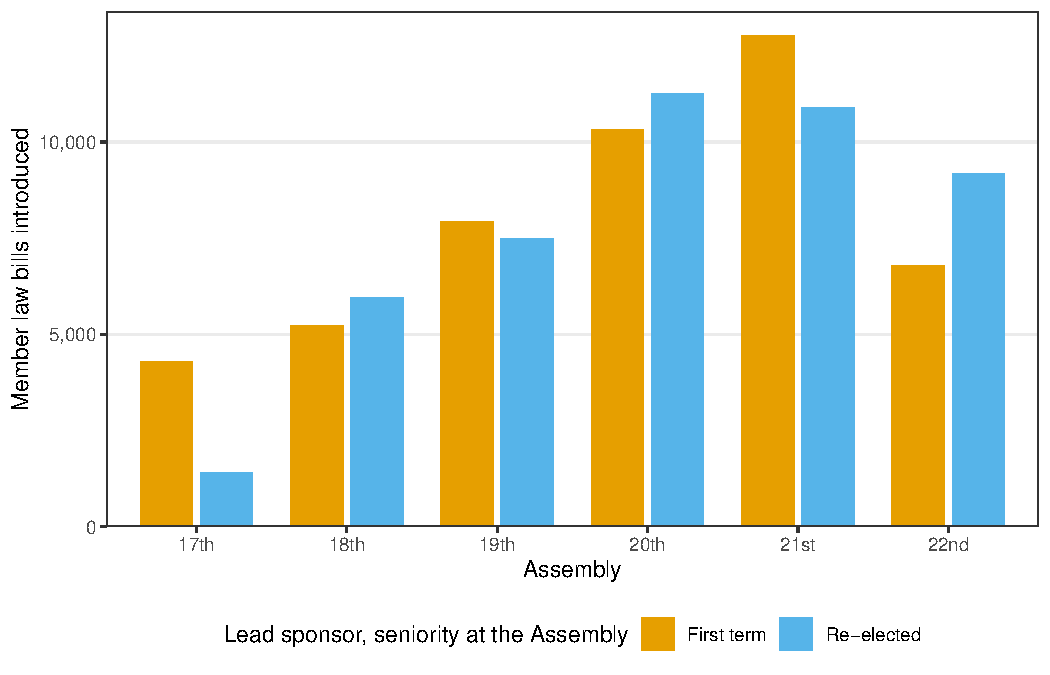
\includegraphics[width=\textwidth]{figures/2026-08-24_r30/fig_1.pdf}
\caption{Member law bills introduced by first-term and re-elected lead sponsors, 17th through 22nd National Assemblies. Seniority is measured at each Assembly.}
\label{fig:volume}
\end{figure}

\subsection{Empirical Strategy}
\label{sec:strategy}

The core estimating equation is a linear probability model of bill outcomes on first-term status interacted with the within-term clock:

\begin{equation}
Y_{icat} = \beta_1 \text{FT}_{i} + \beta_2 \left(\text{FT}_{i} \times \text{Late}_{t}\right) + \lambda_t + \delta_c + \gamma_a + \mathbf{X}_i'\boldsymbol{\theta} + \epsilon_{icat}
\label{eq:main}
\end{equation}

where $Y_{icat}$ is 100 times an indicator that bill $i$, referred to committee $c$ in Assembly $a$ and proposed in term year $t$, achieves the outcome in question (strict passage or absorption into a committee alternative without direct passage). $\text{FT}_i$ indicates a first-term lead sponsor, $\text{Late}_t$ indicates proposal years two through four, $\lambda_t$ are flexible proposal-year effects, $\delta_c$ and $\gamma_a$ are committee and Assembly fixed effects, and $\mathbf{X}_i$ contains sponsor controls for party bloc and election type (district or proportional representation). Standard errors are clustered by lead sponsor. The coefficient $\beta_1$ captures any first-term level gap in year one, and $\beta_2$ captures the average late-term gap. A companion specification replaces the step with separate interactions for years two, three, and four, so that the step form can be compared with a linear trajectory rather than assumed. The step and linear forms are compared with the Bayesian information criterion under flexible year main effects, and the equality of the per-year interactions is assessed with a Wald test. One methods note is required for transparency. An initial information-criterion comparison in Version 1 restricted the proposal-year main effects and favored the linear form by a wide margin, but it confounded the shape of the interaction with the time-trend control and is superseded by the flexible specification. Under the flexible specification the criterion favored the step in the Version 1 coding and favors the linear form in the corrected coding, and neither margin is large (Table~\ref{tab:coding}).

Because the central claims include null results, the design aims to affirm nulls rather than merely fail to reject them. Following the equivalence-testing framework of \citet{hartman2018}, I apply two one-sided tests to the year-one strict-passage gap. Version 1 used a margin of two percentage points. It was proposed at the end of the first round, after the estimated interval for the year-one gap had already excluded gaps of that size, and the test ran in the second round, so it was not an independent test. That margin is not small in relative terms. Against a strict base rate of 6.2 percent, a two-point gap would be roughly a one-third relative deficit. Following the logic of the smallest substantively meaningful effect \citep{rainey2014}, I therefore also report the tighter margin of one point, and I do not rest the no-gap conclusion on an equivalence result alone. That conclusion rests on the conjunction of the bound with a year-one point estimate within a fraction of a point of zero and a within-term trajectory that does not turn against first-term sponsors in the pooled estimates. The project recorded its predictions and thresholds in time-stamped files that it kept itself, and no entry exists at any public registry. Four hypotheses failed their recorded tests, the learning prediction H1, the positional prediction H2b, and the network and portfolio predictions H3 and H4. H2a had no recorded threshold and is not in that count, although the data do not support it. Several auxiliary predictions held under the Version 1 coding, among them the step form, the equivalence of the year-one strict gap within two points, and the absence of deepening at the two-year reconstitution boundary. Under the corrected coding the step form no longer holds. One auxiliary prediction, that the year-one absorption term would be below one point in absolute value, was missed under the Version 1 coding and holds under the corrected coding.

Five threats to inference deserve explicit treatment. First, cohort composition. First-term status is not as-if random. Party nomination strategies, the district-versus-list route into the chamber, age, and prior political careers all differ across cohorts and plausibly across Assemblies. Re-elected members are by construction electoral survivors, so any unobserved ability that raises both re-election odds and legislative success is concentrated in the comparison group. Selection of this kind threatens the late-term gap and not only the level. If survivor ability matters more for absorption as the term progresses, selection alone could generate a late-term deficit. The Version 1 coding compounded this problem by also selecting the first-term group on whether its members later returned to the Assembly. The sponsor controls absorb the party-bloc and seat-type components, but ability selection is unobserved, and I interpret every estimate as a conditional association. Second, committee composition. First-term members may sit on committees that produce fewer or later alternatives, in which case a deficit would be positional \citep{krutz2005}. I address this with committee fixed effects throughout and, in the Version 1 analysis, with a reweighting estimator that assigns first-term bills the re-elected cohort's Assembly-by-committee distribution and a direct accounting of the timing and size of consolidation events. The reweighting operates at the standing-committee level, and subcommittee rosters are not available in the processed data. Third, entry timing. Members seated mid-term through by-elections start their term clock late. Exact seating dates are not in the processed data, and the Version 1 analysis used a behavioral proxy, flagging the 10.3 percent of lifetime-coded first-term sponsor-terms whose first bill appears more than 12 months into the term. Fourth, truncation. The 22nd Assembly's later years are unobserved, and bills proposed late in an ongoing term mechanically lack time to pass or be absorbed. That shortfall is specific to late proposal years within one Assembly, which an Assembly intercept cannot absorb. I therefore re-estimate excluding the 22nd Assembly and report per-Assembly estimates. Fifth, the outcome definition itself. Because the definitional choice moves the passage rate by a factor of five, the headline results are reported under both definitions. Throughout, the design is selection on observables, and the estimates identify associations between cohort and bill outcomes conditional on the stated controls.

A final design point concerns the mechanism tests. Cosponsor rosters and portfolio content are measured after, and chosen jointly with, first-term status, so conditioning on them is conditioning on post-treatment variables. Each test is informative under a stated assumption. The network and portfolio tests treat roster composition and statute choice as candidate mediators of a cohort-absorption association, and they ask whether the data show the two signatures mediation requires, a first stage that exists and conditioning that attenuates. If a conditioning variable is instead a collider, affected by cohort and by unobserved determinants of absorption, conditioning could distort the estimate in either direction, and the distortion is not identifiable from these data. The network verdict does not depend on conditioning, because the account fails at the unconditional first stage. The portfolio result in which conditioning enlarges the gap is read descriptively, not as a causal decomposition.

\section{Results}

\subsection{No Gap on Strict Passage}

The learning hypothesis fails at its premise. Figure~\ref{fig:null} plots raw strict passage rates of member law bills by sponsor cohort in each Assembly, with seniority measured at the Assembly. The two series are close in four of the six Assemblies. In the 19th and the 21st, first-term sponsors' raw rates are lower, by about two and a half and one percentage points, before any adjustment for committee, party bloc or proposal year. Table~\ref{tab:coding} reports the regression estimates under both codings. With Assembly and committee fixed effects and sponsor controls, the year-one gap in strict passage between first-term and re-elected sponsors is a fraction of a percentage point under either coding, and neither estimate is distinguishable from zero. The linear interaction of first-term status with the proposal year is close to zero under both codings. No pooled specification produces a strict-passage deficit for first-term sponsors at any point in the term. The per-Assembly interactions, in Table~\ref{tab:perassembly}, are mostly small. The 17th Assembly shows a decline for first-term sponsors over the term under both codings, and the 20th shows a rise.

Because these are null claims, I test them for equivalence rather than resting on insignificance. Under the corrected coding, the two one-sided tests reject any year-one gap larger than one percentage point in either direction at the 5 percent level, and a fortiori any gap larger than two points. One point is about one sixth of the strict passage rate. A margin of one tenth of the base rate, about 0.6 points, is not attained, as the 90 percent interval in Table~\ref{tab:coding} shows. Under the Version 1 coding equivalence held at two points but not at one. H1 is not supported, and its premise, a gap for learning to close, finds no support anywhere in the term.

\begin{figure}[H]
\centering
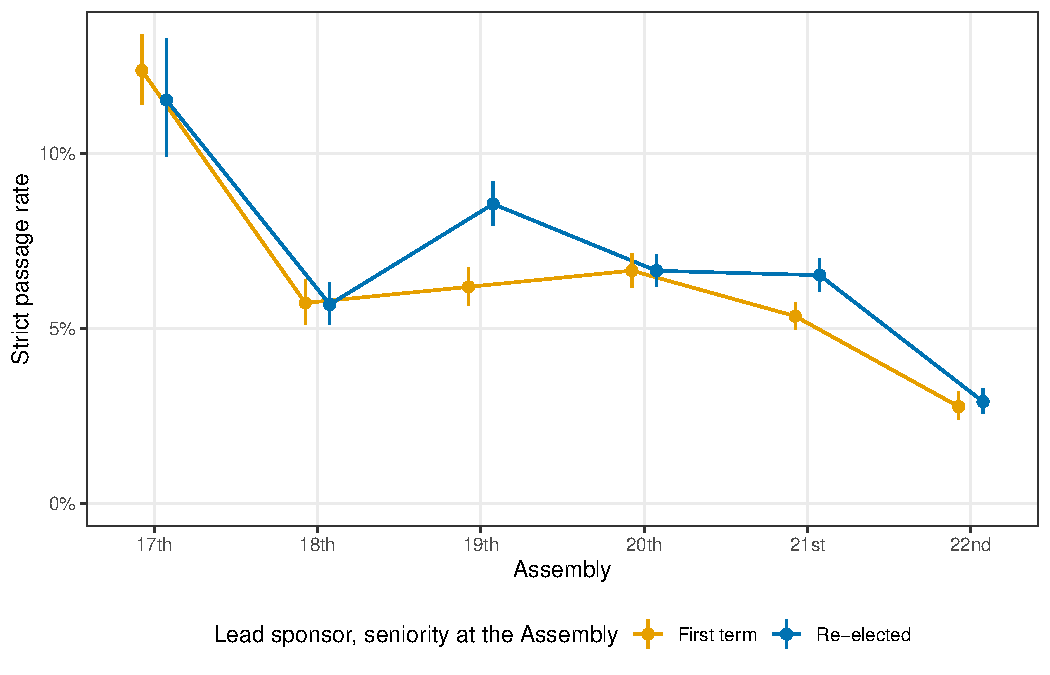
\includegraphics[width=\textwidth]{figures/2026-08-24_r30/fig_2.pdf}
\caption{Strict passage rates of member law bills by lead sponsor's seniority at the Assembly, 17th through 22nd Assemblies, with exact 95 percent binomial confidence intervals. Strict passage counts bills enacted in original or amended form.}
\label{fig:null}
\end{figure}

Figure~\ref{fig:ladder} places the cohort comparison on the full seniority ladder, plotting raw strict passage rates for first-, second-, third-term, and more senior sponsors pooled across the six Assemblies, with binomial confidence intervals. First-, second- and third-term sponsors pass bills at similar raw rates, near 6 percent, and members in their fourth term or later at a slightly lower rate. Whatever seniority buys in this legislature, the direct-passage margin is not where it visibly accumulates.

\begin{figure}[H]
\centering
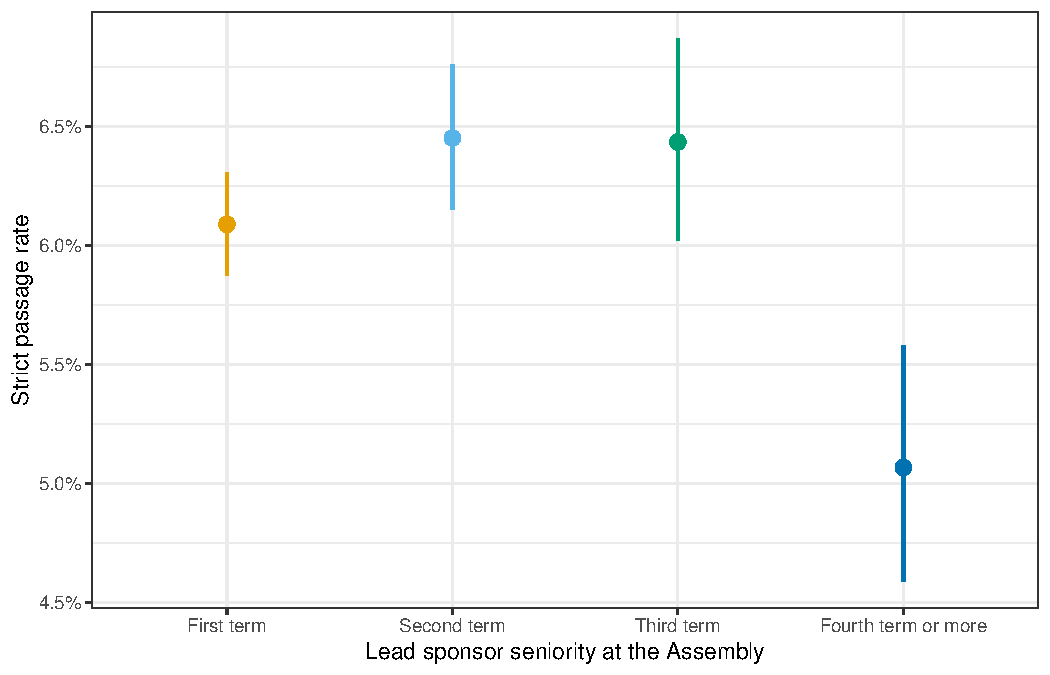
\includegraphics[width=\textwidth]{figures/2026-08-24_r30/fig_3.pdf}
\caption{Strict passage rates by lead sponsor's seniority at the Assembly, member law bills of the 17th through 22nd Assemblies pooled, with exact 95 percent binomial confidence intervals.}
\label{fig:ladder}
\end{figure}

\subsection{The Absorption Channel Under Two Codings}

The picture differs on the absorption channel, and it differs by coding. The absorption pattern was not predicted, and the results in this subsection and the next two are exploratory. Table~\ref{tab:coding} reports Equation~\ref{eq:main} with absorption into a committee alternative as the outcome. With seniority measured at the Assembly, first-term sponsors' bills are absorbed at about the re-elected rate in year one. From year two onward they are on average about one and a half percentage points less likely to be absorbed, and that average is not distinguishable from zero at the 5 percent level. The per-year interactions grow from about one point in year two to about three points in year four, and only the year-four interaction is distinguishable from zero. The linear trend in the interaction is distinguishable from zero, the information criterion favors the linear form over the step, and the three per-year interactions cannot be told apart statistically. Two of the variants reach the 5 percent level, the model that excludes the truncated 22nd Assembly and the model that weights member-periods equally. Against an absorption rate of about 25 percent, a gap of one and a half points is modest. Taken together, these estimates suggest a small absorption disadvantage for first-term sponsors that widens over the term, and they need to be interpreted with caution. H2a, which expected no first-term absorption deficit at any point in the term, is not supported. Under the corrected coding the year-four interaction and the linear trend are distinguishable from zero at the 5 percent level, and under the Version 1 coding every late-term estimate is. H2a had no recorded threshold, so it is not counted among the hypotheses that failed a recorded test.

Under the Version 1 coding the same models give a larger and differently shaped gap. The average late-term gap is about three and a half percentage points, the per-year interactions are flat across years two to four at roughly three to four and a half points, and the information criterion favors the step. The year-one term is positive, about one and a half points, and carries one star at the 10 percent level. Table~\ref{tab:main} reports the Version 1 main models with their standard errors. The difference between the two codings comes from the 18,969 bills of first-term members who were later re-elected, which Version 1 counted in the comparison group. For the 17th through 21st Assemblies, the Version 1 step therefore compares members who had served only one term as of the collection date with all other members, and it cannot be read as a property of first-term status. The next two subsections report the Version 1 analyses of that step, which were not re-estimated under the corrected coding.

\begin{table}[H]
\centering
\singlespacing
\caption{Headline Estimates Under Two Codings of First-Term Status}
\label{tab:coding}
\small
\begin{tabular}{p{0.56\textwidth}cc}
\toprule
& (1) & (2) \\
& Corrected coding & Version 1 coding \\
& (at the Assembly) & (lifetime count) \\
\midrule
Strict passage, year-1 bills: first term & $-0.21$ & $0.24$ \\
& (0.47) & (0.54) \\
Strict passage: first term $\times$ proposal year (linear) & $0.01$ & $-0.06$ \\
& (0.24) & (0.28) \\
Absorption: first term (year 1) & $0.46$ & $1.42^{*}$ \\
& (0.78) & (0.83) \\
Absorption: first term $\times$ late term & $-1.51^{*}$ & $-3.50^{***}$ \\
& (0.89) & (0.89) \\
Absorption: first term $\times$ year 2 & $-0.86$ & $-3.21^{***}$ \\
& (1.04) & (1.01) \\
Absorption: first term $\times$ year 3 & $-1.51$ & $-3.29^{***}$ \\
& (1.16) & (1.15) \\
Absorption: first term $\times$ year 4 & $-2.89^{**}$ & $-4.55^{***}$ \\
& (1.32) & (1.30) \\
Absorption: first term $\times$ proposal year (linear) & $-0.89^{**}$ & $-1.52^{***}$ \\
& (0.41) & (0.41) \\
Absorption step, single late-term indicator & $-1.51^{*}$ & $-2.97^{***}$ \\
& (0.89) & (0.88) \\
Absorption step, excluding the 22nd Assembly & $-2.10^{**}$ & $-2.90^{***}$ \\
& (1.00) & (1.07) \\
Absorption step, member-period cells ($n \geq 3$) & $-1.99^{**}$ & $-2.28^{**}$ \\
& (0.99) & (1.02) \\
\midrule
N (bills), year-1 model & 34,652 & 34,652 \\
N (bills), full-term models & 93,078 & 93,078 \\
N (member-period cells) & 3,423 & 3,423 \\
N (bills), excluding the 22nd & 77,188 & 77,188 \\
N (lead sponsors, clusters) & 1,128 & 1,128 \\
\midrule
\multicolumn{3}{l}{\textit{Tests}} \\
Equivalence, year-1 strict gap within $\pm 2$ points, largest one-sided $p$ & 0.0001 & 0.0005 \\
Equivalence, year-1 strict gap within $\pm 1$ point, largest one-sided $p$ & 0.046 & 0.077 \\
90 percent interval of the year-1 strict gap & $-0.98$ to $0.55$ & $-0.64$ to $1.12$ \\
Equality of the year 2, 3 and 4 absorption interactions, Wald $p$ & 0.276 & 0.529 \\
BIC of the step model minus BIC of the linear model & $4.6$ & $-4.3$ \\
\bottomrule
\end{tabular}

\smallskip
\begin{minipage}{0.95\textwidth}
\footnotesize $^{*}p<0.10$, $^{**}p<0.05$, $^{***}p<0.01$. Outcomes are indicators scaled by 100, so estimates are in percentage points. The absorption outcome is absorption into a committee alternative without direct passage. Standard errors, clustered by lead sponsor, in parentheses. Column 1 measures first-term status as the term number at the Assembly (Section~\ref{sec:coding}). Column 2 uses the Version 1 lifetime coding. The strict year-one model uses year-one bills. The absorption models of the first block use proposal-year effects, except the rows labeled single late-term indicator, which replace them with one late-term indicator. All models include Assembly and committee fixed effects and sponsor controls, except the member-period cell model, which has no committee fixed effects. The linear strict interaction uses $t$-based inference as in the original script. Equivalence tests use a normal reference distribution, and the 90 percent interval is the one the two one-sided tests compare with the margins.
\end{minipage}
\end{table}

\begin{table}[H]
\centering
\singlespacing
\caption{Per-Assembly Estimates Under Two Codings of First-Term Status}
\label{tab:perassembly}
\small
\begin{tabular}{lcccc}
\toprule
& \multicolumn{2}{c}{Strict passage trend} & \multicolumn{2}{c}{Absorption step} \\
& (1) & (2) & (3) & (4) \\
& Corrected & Version 1 & Corrected & Version 1 \\
\midrule
17th Assembly, N = 5,721 & $-3.66^{*}$ & $-2.74^{**}$ & $4.35$ & $4.90$ \\
& (2.00) & (1.28) & (3.22) & (3.75) \\
18th Assembly, N = 10,818 & $-0.99^{*}$ & $-0.75$ & $-4.19^{*}$ & $-2.91$ \\
& (0.58) & (0.58) & (2.45) & (2.52) \\
19th Assembly, N = 15,435 & $-0.21$ & $0.50$ & $-2.42$ & $-2.93$ \\
& (0.47) & (0.60) & (1.87) & (2.24) \\
20th Assembly, N = 21,590 & $1.14^{**}$ & $1.22^{*}$ & $-1.67$ & $-6.36^{***}$ \\
& (0.50) & (0.70) & (1.98) & (2.00) \\
21st Assembly, N = 23,624 & $0.17$ & $-0.18$ & $-2.19$ & $-2.17$ \\
& (0.40) & (0.45) & (1.58) & (1.83) \\
22nd Assembly, N = 15,890 & $-0.01$ & $-0.01$ & $-0.41$ & $-0.41$ \\
& (0.58) & (0.58) & (1.43) & (1.43) \\
\bottomrule
\end{tabular}

\smallskip
\begin{minipage}{0.95\textwidth}
\footnotesize $^{*}p<0.10$, $^{**}p<0.05$, $^{***}p<0.01$. Estimates in percentage points, standard errors clustered by lead sponsor in parentheses. Columns 1 and 3 use the corrected coding (seniority at the Assembly), and columns 2 and 4 the Version 1 lifetime coding. Columns 1 and 2 are the linear interaction of first-term status with the proposal year on strict passage, with $t$-based inference. Columns 3 and 4 are the late-term absorption step with a single late-term indicator. Each model is fitted within one Assembly, with committee fixed effects and sponsor controls. The two codings agree in the 22nd Assembly.
\end{minipage}
\end{table}

\begin{table}[H]
\centering
\singlespacing
\caption{Version 1 Main Models, Lifetime Coding of First-Term Status}
\label{tab:main}
\small
\begin{tabular}{lcccc}
\toprule
& (1) & (2) & (3) & (4) \\
& Strict passage & Absorption & Absorption & Absorption \\
& (year-1 bills) & (step) & (per year) & (member-period cells) \\
\midrule
First term (lifetime coding) & $0.24$ & $1.42^{*}$ & $1.42^{*}$ & $1.30$ \\
& (0.54) & (0.83) & (0.83) & (0.96) \\
First term $\times$ late term & & $-3.50^{***}$ & & $-2.28^{**}$ \\
& & (0.89) & & (1.02) \\
First term $\times$ year 2 & & & $-3.21^{***}$ & \\
& & & (1.01) & \\
First term $\times$ year 3 & & & $-3.29^{***}$ & \\
& & & (1.15) & \\
First term $\times$ year 4 & & & $-4.55^{***}$ & \\
& & & (1.30) & \\
\midrule
Assembly fixed effects & Yes & Yes & Yes & Yes \\
Committee fixed effects & Yes & Yes & Yes & No \\
Sponsor controls & Yes & Yes & Yes & Yes \\
Proposal-year effects & No & Yes & Yes & No \\
Late-term indicator & No & No & No & Yes \\
N & 34,652 & 93,078 & 93,078 & 3,423 \\
Clusters (lead sponsors) & 1,051 & 1,128 & 1,128 & 1,104 \\
\bottomrule
\end{tabular}

\smallskip
\begin{minipage}{0.95\textwidth}
\footnotesize $^{*}p<0.10$, $^{**}p<0.05$, $^{***}p<0.01$. First-term status uses the Version 1 lifetime coding, which for the 17th through 21st Assemblies marks only first-term members who were never re-elected. Outcomes are indicators scaled by 100, so estimates are in percentage points. Standard errors, clustered by lead sponsor, in parentheses. Column 4 averages the absorption outcome within member-by-period cells (year one and years two to four) that hold at least three bills, weights cells equally, and counts cells in its N. In column 3, a Wald test cannot reject equality of the three late-term interactions (Table~\ref{tab:coding}).
\end{minipage}
\end{table}

The definitional point follows from the two outcomes. Under the strict definition no cohort difference appears anywhere in the pooled estimates. Under the absorption definition a gap appears that widens over the term. Because the two definitions differ by a factor of five in level and disagree in what they detect, a study of Korean legislative effectiveness should state which disposition codes count as success. Whether published Korean studies of seniority \citep{an2025, jeong2016, ka2025a} count absorbed bills as successes could not be established from their abstracts, and I did not read their full texts, so whether their findings depend on this choice is untested.

\subsection{Version 1 Robustness of the Step}

Table~\ref{tab:robust} reports the artifact checks that Version 1 ran on the step, all with the lifetime coding. Most rows use a single late-term indicator instead of proposal-year effects, and their full-sample counterpart is the second row, not the first. The positional test of H2b is the most consequential. Reweighting lifetime-coded first-term bills to the re-elected cohort's Assembly-by-committee distribution moves the single-indicator step by one hundredth of a percentage point. The threshold written down for H2b was attenuation of at least half, and the observed attenuation is zero at the standing-committee level. The regression version of this check is weak by construction, because the baseline already includes committee fixed effects, so reweighting can move the estimate only through differences in the step across committees. The raw cell double difference, which has no committee controls, is the more informative version, and reweighting moves it by less than a tenth of a point.

The timing account fares no better. Year-one consolidation activity is not thin. In the first year of the term, 393 processing events handled 4,138 absorbed bills, of which 1,158 had lifetime-coded first-term sponsors. Of the bills these sponsors proposed in year one, 29.3 percent were absorbed at some point, against 29.2 percent for other sponsors, and 82 percent of year-one-proposed absorbed bills are processed within the first two years of the term. Nor does the year-one parity reflect first-term bills being swept into unusually large early omnibus packages. The median consolidation event sizes for the two groups are 20 and 21 bills, and the mean sizes, 36.2 and 39.6, run slightly against the first-term group.

The remaining rows probe composition and truncation. The step is negative within every estimated cosponsor-coalition size bin and is largest for small coalitions. These bins are estimable only for the 20th through 22nd Assemblies and cover about two thirds of all bills in the panel. Excluding sponsors whose first bill appears more than 12 months into the term leaves the step essentially unchanged, as does excluding the truncated 22nd Assembly. The per-Assembly estimates are negative in five of six Assemblies, individually distinguishable from zero only in the 20th, near zero in the still-running 22nd, and positive only in the 17th, where the estimate is imprecise. These checks indicate that committee mix, event timing, event size, heavy sponsors, late entrants and truncation do not account for the Version 1 step. They do not address the coding problem, which none of them varies.

\begin{table}[H]
\centering
\singlespacing
\caption{Version 1 Robustness of the Absorption Step, Lifetime Coding}
\label{tab:robust}
\small
\begin{tabular}{lc}
\toprule
Specification & Estimate \\
\midrule
Step with proposal-year effects (Table~\ref{tab:main}, column 2), N = 93,078 & $-3.50^{***}$ \\
& (0.89) \\
Step with a single late-term indicator, N = 93,078 & $-2.97^{***}$ \\
& (0.88) \\
\quad reweighted to the re-elected committee distribution, N = 93,078 & $-2.96^{***}$ \\
& (0.90) \\
Raw cohort double difference, N = 93,078 & $-2.39^{***}$ \\
& (0.90) \\
\quad reweighted, N = 93,078 & $-2.44^{***}$ \\
& (0.92) \\
Member-period cells, equal weights ($n \geq 3$), N = 3,423 cells & $-2.28^{**}$ \\
& (1.02) \\
Excluding late-starting sponsors (clock proxy), N = 92,067 & $-2.91^{***}$ \\
& (0.89) \\
Excluding the 22nd Assembly, N = 77,188 & $-2.90^{***}$ \\
& (1.07) \\
Edge-covered subsample, 20th to 22nd, N = 60,684 & $-3.63^{***}$ \\
& (1.03) \\
\midrule
Coalition of 10 or fewer sponsors, N = 25,733 & $-4.76^{***}$ \\
& (1.75) \\
Coalition of 11 to 15 sponsors, N = 28,263 & $-2.88^{**}$ \\
& (1.29) \\
Coalition of 16 to 30 sponsors, N = 5,692 & $-2.57$ \\
& (2.77) \\
\midrule
17th Assembly only, N = 5,721 & $4.90$ \\
& (3.75) \\
18th Assembly only, N = 10,818 & $-2.91$ \\
& (2.52) \\
19th Assembly only, N = 15,435 & $-2.93$ \\
& (2.24) \\
20th Assembly only, N = 21,590 & $-6.36^{***}$ \\
& (2.00) \\
21st Assembly only, N = 23,624 & $-2.17$ \\
& (1.83) \\
22nd Assembly only, N = 15,890 & $-0.41$ \\
& (1.43) \\
\bottomrule
\end{tabular}

\smallskip
\begin{minipage}{0.95\textwidth}
\footnotesize $^{*}p<0.10$, $^{**}p<0.05$, $^{***}p<0.01$. Estimates are the late-term absorption gap of lifetime-coded first-term sponsors, in percentage points. Standard errors, clustered by lead sponsor, in parentheses. Every row except the first uses a single late-term indicator in place of proposal-year effects. The raw double differences have no controls, and their standard errors come from the equivalent saturated regression. The reweighted rows weight lifetime-coded first-term bills to the re-elected Assembly-by-committee distribution, with weights capped at 10. Coalition-size bins are estimable only for the 20th through 22nd Assemblies, and the bin with more than 30 sponsors, 996 bills, was not estimated. Per-Assembly rows drop the Assembly effects.
\end{minipage}
\end{table}

\subsection{Version 1 Mechanism Tests}

Table~\ref{tab:mech} reports the mechanism tests for H3 and H4 and the assignment-timing shape check, all run in Version 1 with the lifetime coding. Each test had a directional prediction and, where relevant, a 50 percent attenuation threshold written down before it ran. The incumbent share in Panel A counts as incumbents the cosponsors whose lifetime seniority exceeds one term, so it also counts first-term cosponsors who were later re-elected. The post-treatment caveat of Section~\ref{sec:strategy} applies to every conditional estimate in this subsection.

Panel A takes up the network-access account. Its first requirement, that the incumbent share of first-term sponsors' cosponsor rosters falls after year one, is not met. The share is flat within first-term bills, and the cohort difference in differences shows first-term rosters becoming relatively more incumbent-heavy late in the term, the opposite of decay. The account's second requirement also fails. The incumbent share of a bill's roster does not predict absorption, in the full edge-covered sample or within first-term bills. With no first stage, no configuration of share dynamics could transmit the step, and because the first stage is estimated without conditioning on anything post-treatment, this verdict does not depend on the mediator assumptions. Conditioning agrees. Adding the incumbent share and coalition size attenuates the step by 3 percent against the 50 percent threshold, and within-committee share-decile fixed effects attenuate it by less than 2 percent. The share path has one granular feature. The first-term incumbent share dips modestly in year two before rising above its year-one level in years three and four, but a share that does not predict absorption cannot transmit a dip of any timing. Lifetime-coded first-term rosters carry about 11 percentage points fewer incumbent cosigners than other sponsors' rosters in years one and two, and the gap narrows to about 4 to 5 points in years three and four.

Panel B takes up the portfolio-content account, and here the conditioning runs the other way. The contemporaneous duplicate measure, whether a first-term bill's base statute also carries a same-committee incumbent bill in the same Assembly, sits near 90 percent in every proposal year and moves the step by a fraction of a percent when conditioned upon. Because the measure has almost no variation, this null is weakly informative. The temporally ordered measure is more informative. Whether a prior incumbent bill exists on the same statute rises mechanically over the term as the stock accumulates, from about 76 to about 89 percent of first-term bills, predicts absorption, and, when conditioned upon, makes the step larger by about 28 percent. Lifetime-coded first-term members increasingly write bills on the statutes where consolidation activity concentrates, and accounting for this enlarges rather than shrinks their late-term gap. Because statute choice is a post-treatment variable, the amplification is read as descriptive evidence about where these bills sit in the consolidation landscape, not as a causal decomposition, and a collider reading cannot be ruled out. The new-enactment composition check points the same way. The first-term share of bills proposing new statutes moves little across the term, drifts slightly toward new statutes relative to other sponsors, and explains almost none of the step. Jointly, the network and portfolio controls enlarge the step by 19 percent rather than shrinking it. H4 is not supported.

Panel C reports the assignment-timing shape check. If subcommittee or committee position drove the step through the two-year reconstitution calendar, the gap should deepen at the year-two to year-three boundary, when positions are reallocated. The estimated deepening is less than a tenth of a percentage point, and the per-year interactions are jointly flat. Because subcommittee rosters are unmeasured, I state this as shape inconsistency rather than as a refutation.

\begin{table}[H]
\centering
\singlespacing
\caption{Version 1 Mechanism Tests, Lifetime Coding: Network Access, Portfolio Content, and Assignment Timing}
\label{tab:mech}
\small
\begin{tabular}{lc}
\toprule
& Estimate \\
\midrule
\multicolumn{2}{l}{\textit{Panel A: Cosponsorship network (20th to 22nd Assemblies)}} \\
Incumbent share, first-term bills, late term vs.\ year 1, N = 18,996 & $-0.35$ \\
& (0.64) \\
Incumbent share, cohort difference in differences, N = 60,684 & $2.25^{***}$ \\
& (0.85) \\
Absorption on incumbent share, all bills (first stage), N = 60,684 & $0.05$ \\
& (1.45) \\
Absorption on incumbent share, first-term bills, N = 18,996 & $-0.46$ \\
& (2.28) \\
Absorption step, unconditional, N = 60,684 & $-3.63^{***}$ \\
& (1.03) \\
Absorption step, conditional on share and coalition size, N = 60,684 & $-3.52^{***}$ \\
& (1.03) \\
Absorption step, within-committee share-decile fixed effects, N = 60,683 & $-3.57^{***}$ \\
& (1.03) \\
\midrule
\multicolumn{2}{l}{\textit{Panel B: Portfolio content (17th to 22nd Assemblies)}} \\
Contemporaneous same-statute duplicate, first-term bills, late vs.\ year 1, N = 28,350 & $0.55$ \\
& (0.47) \\
Absorption step, conditional on the contemporaneous duplicate, N = 93,078 & $-2.97^{***}$ \\
& (0.88) \\
Absorption on a prior incumbent bill on the same statute, N = 93,078 & $7.13^{***}$ \\
& (0.74) \\
Absorption step, unconditional (single late-term indicator), N = 93,078 & $-2.97^{***}$ \\
& (0.88) \\
Absorption step, conditional on the prior duplicate, N = 93,078 & $-3.79^{***}$ \\
& (0.88) \\
New-enactment share, cohort difference in differences, N = 93,078 & $1.44^{***}$ \\
& (0.41) \\
Absorption step, conditional on new enactment, N = 93,078 & $-2.89^{***}$ \\
& (0.88) \\
Absorption step, joint controls (edge-covered subsample), N = 60,684 & $-4.32^{***}$ \\
& (1.03) \\
\midrule
\multicolumn{2}{l}{\textit{Panel C: Assignment-timing shape (17th to 22nd Assemblies)}} \\
Step deepening at the year-3 boundary (year 3 minus year 2), N = 93,078 & $-0.08$ \\
& (1.14) \\
\bottomrule
\end{tabular}

\smallskip
\begin{minipage}{0.95\textwidth}
\footnotesize $^{*}p<0.10$, $^{**}p<0.05$, $^{***}p<0.01$. First-term status uses the Version 1 lifetime coding. Outcomes are indicators scaled by 100, so estimates are in percentage points, and incumbent share enters as a proportion. Standard errors, clustered by lead sponsor, in parentheses. Incumbent share is the share of a bill's cosponsors, excluding the lead sponsor, whose lifetime seniority exceeds one term. Network quantities are estimable only where cosponsorship edges are identifier-linked, 99.3 percent of bills in the 20th through 22nd Assemblies. Step models use a single late-term indicator. Attenuation, reported in the text, is the change in the step relative to the unconditional step in the same sample.
\end{minipage}
\end{table}

Taken together, the Version 1 mechanism tests leave the Version 1 step with none of its three measured explanations supported, each judged against its own threshold. Committee-level position shows zero attenuation, the cosponsorship-network account has no first stage and no share decay, and the portfolio controls amplify rather than attenuate. These tests render the candidate mechanisms implausible under the available measures for the lifetime-coded contrast. They do not exclude them in any strict sense, because observational conditioning cannot rule out unmeasured versions of each channel. Whether the same tests would behave the same way for the smaller gap under the corrected coding is untested.

\section{Discussion}

The learning account entered the analysis as the prior and exits with its within-term premise unsupported under either coding, since there is no first-term deficit in direct passage for experience to remedy. The verdict is scoped to the cohort comparison the design estimates. Learning shared by both cohorts, or learning completed before entry through prior political careers, would leave the same null, so the data speak against the version of the account in which chamber tenure separates the cohorts, not against the relevance of experience to legislating in general.

The absorption results call for more caution than Version 1 applied. With seniority measured at the Assembly, first-term sponsors fall behind on absorption as the term goes on, but the average gap is small and not distinguishable from zero at the 5 percent level, and its shape is closer to a gradual decline than to a step. For the 17th through 21st Assemblies, the larger step of Version 1 compared members who had served only one term as of the collection date with everyone else. That group is defined partly by whether its members later returned to the Assembly, so its step cannot be attributed to first-term status, and I do not offer an account of it here.

The comparison with \citet{casas2020} is best stated as a tentative contrast. They report that counting hitchhiker bills as sponsorship successes reveals a less hierarchical and less partisan lawmaking process in the United States Congress. The Korean evidence here does not show absorption favoring first-term members. The two findings are not directly comparable. Casas, Denny and Wilkerson describe how legislative success is distributed across sponsors once hitchhikers are counted, while this paper estimates how one cohort's absorption rate changes within a term relative to another cohort's. Differences in how consolidation is organized, such as the chair-assembled Korean alternative against provisions carried in other vehicles, may matter for such a contrast, but that is a conjecture for comparative work, not a finding of this paper.

The positional, network and portfolio results bear on the Version 1 step only. The committee-level positional test is weak in its regression form, and the operative variable in \citet{kim2023}, subcommittee membership, lies one level below every control in this paper, so the positional account is not rejected at the subcommittee level. The flat reconstitution boundary is a shape argument against assignment timing, not a test of subcommittee position. The network results differ from what the connectedness literature would lead one to expect \citep{battaglini2020, fowler2006}, since the incumbent composition of a bill's coalition does not predict absorption here, but the incumbent share itself uses the lifetime field. The portfolio results show the lifetime-coded first-term bills concentrating on statutes where consolidation happens, which runs against the portfolio account's prediction of a drift toward position-taking content, and the conditioning involved is post-treatment.

Several limitations bound the claims, and I state them in descending order of threat. First, the corrected coding changes the absorption result, and the robustness and mechanism analyses were not re-estimated under it, so they describe the lifetime-coded contrast only. Second, first-term status is not as-if random, and re-elected members are a selected set of electoral survivors under either coding. If unobserved survivor ability matters more for absorption late in the term, selection could contribute to any late-term gap, and no control in the analysis rules this out. Third, subcommittee position is unmeasured. Fourth, the network tests cover the 20th through 22nd Assemblies, where cosponsorship edges are identifier-linked, and the network channel in the 17th through 19th is unobserved. Fifth, the portfolio measures are statute-level rather than text-level, and a text-level measure could detect content differences invisible to statute matching. Sixth, entry timing rests on a behavioral proxy. Seventh, the 22nd Assembly is truncated, and its estimates should be read as weak evidence from an incomplete term. Eighth, the absorption hypotheses were formulated after the pattern was seen, and the project's records of its predictions were kept by the project itself. Finally, the design is observational throughout, and no estimate here is a causal effect of first-term status.

\section{Conclusion}

This paper asked whether first-term members of the Korean National Assembly underperform, whether any deficit closes with experience, and through which channel seniority pays. With seniority measured at each Assembly, first-term sponsors pass bills directly at the same rate as their re-elected colleagues at the start of the term and across it, and the year-one gap is bounded within one percentage point of zero. The learning account has no observed gap to explain. On the committee-alternative channel, first-term sponsors' bills are absorbed at about the re-elected rate in year one and fall behind as the term goes on, but the average gap after year one is about one and a half points and is not distinguishable from zero at conventional levels. The larger step reported in Version 1 belonged to a coding that selected first-term members on whether they later returned to the Assembly, and the mechanism tests of Version 1 speak to that coding only.

The study has two lessons for measurement. The strict and absorption-inclusive definitions of passage differ by a factor of five and detect different things, so any study of Korean legislative effectiveness should state which disposition codes count as success. A seniority field recorded at collection must not be read as seniority at an earlier Assembly, because it sorts members by their later careers.

Future research has a concrete agenda. The Version 1 robustness and mechanism analyses can be rerun under the corrected coding. Subcommittee rosters for the 17th through 22nd Assemblies would allow a direct test of the positional account. A text-level measure of absorption would test whether the administrative disposition codes conceal content-level differences, and administrative seating dates would replace the behavioral entry-timing proxy. The Korean evidence supports a modest conclusion. In this legislature, newcomers show no sign of needing time to learn how to pass bills directly, and whether they are at a disadvantage when bills are consolidated into committee alternatives remains an open question.

\bigskip
\noindent\textbf{AI-generation disclosure.} This working paper was generated end to end by an autonomous AI research-agent system (kna-research-agents.com) as an experimental output. Version 2 was corrected by the orchestrating Claude session at the researcher's request after an audit, as the correction notice describes. No human author of record exists, and the authorship line denotes the agent system. This statement is provided to satisfy journal policies on AI-generated content. The paper has not been peer-reviewed or independently fact-checked. Do not cite or use it in any academic, policy, or professional context.

\medskip
\noindent\textbf{Data availability.} All analyses draw on the processed files of the Korean National Assembly legislative database described in Section 3, as they stand at commit 3d8d55d of the main branch of its public repository (github.com/kyusik-yang/kna). The later release kna version 0.7.0 adds the term-number field used in Section~\ref{sec:coding} and also changes the sample, so the numbers here reproduce only on the pinned commit. The scripts that produced every number and figure in this version are in the forum repository's replication package, replication/arc\_5, which holds scripts and no data and lists the checksum of each input file. With those files in the directory named by the KBL\_DATA environment variable, the package rebuilds the analysis panel byte for byte and reproduces every number in Tables~\ref{tab:desc} to \ref{tab:mech}, and it was verified on 26 September 2026. The time-stamped files in which the project recorded its predictions and thresholds are not part of the package. No analysis code appears in the manuscript.

\bibliographystyle{apsr}
\bibliography{references_r30}

\end{document}
